\documentclass[10pt,a4,oneside]{article}
\usepackage{a4wide}
\usepackage{graphicx}

\begin{document}
\title{\textbf{EARTH PROJECT}\\ \textit{} \\ \textit{} \textbf{Milestone 3 Plan}\\ \textit{} \\ \textit{} \textit{for} \\ \textit{} \\ \textit{} \textbf{Group 1}\\ \textit{} \\ \textit{}}
\author{Alex Egan \\ Filimoni Lutunaika \\ George Sainsbury \\ Xiaodong Cui}
 
\maketitle

\newpage

\tableofcontents

\[----\]

\paragraph{}

\listoffigures
 
\newpage

\section{Introduction} 
 
\subsection{Purpose and Scope}

\label{subsec:purpose-and-scope}
 
Milestone 3 follows on the from development tasks undertaken during Milestones 1 and 2. In particular, 
it expands on the investigation done for Ticket 138 issue regarding the unacceptable performance of the 
Earth application when filtering under radial view. In addition, Milestone 3 also involves the investigation 
and possible resolve for the following 2 Tickets:

\subsubsection*{Ticket 148 - Configuration of daemon should be possible through GUI}

The daemon configuration options should be done through the administrative interface of Earth so that 
starting a daemon on a server is as simple as ./earth\_daemon.rb and all options are fed from a central location.

\noindent Of course, this has implications that we should be able to add a server to be indexed through the admin 
interface instead of it being created the first time the daemon runs. 


\subsubsection*{ Ticket 174 - Look into making Earth release a gem}

It would allow us to automatically deal with the dependencies such as:



\begin{itemize}
\item the gems:
  \subitem rcov
  \subitem rails
  \subitem postgres 
\end{itemize}
 
The remove feature of the daemon is also being considered by Group 1 for Milestone 3. 

 
\subsection{Milestone 3 Deliverables}
 
The following section outlines when specific documents and deliverables will be 
completed and available. These are the main deliverables. However, more detailed 
information about internal milestones are provided in subsection \ref{subsec:purpose-and-scope}.
 
\subsection{Evolution of the Plan}
 
This plan will be reviewed at the end of the Milestone 3 development 'sprint'. This plan 
will be updated if there is a radical change to the requirements of any Milestone 3 task. 
The changes can be made by any of the group member who should then inform the group leader 
about these changes. However, significant changes that have a system-wide effect will be deferred 
to the next milestone to minimize any disruption to the other tasks of the current milestone.

\newpage

\section{Organisation for Milestone 3}
 
\label{sec:g1org}

\subsection{Task Allocations}

Tasks for Milestone 3 are being allocated as follow:
 
\subsubsection*{Ticket 138: Query Optimisation for Filtering Under Radial View}
Cui is being re-allocated this task for Milestone 3 given his prior knowledge of this issue while undertaking the same Ticket during Milestone 2.

\noindent Time Estimate: 50hrs
 
\subsubsection*{Ticket 148: Configuration of Daemon using GUI}
Fil is being allocated this task for Milestone 3 to allow for the easy re-configuration of the earthd daemon when switching between the three operating modes of the application, development, test and production. This feature is particularly useful during the integration testing phase where regular switching between the various operating modes will be required.
 
\noindent Time Estimate: 50hrs

\subsubsection*{Ticket 174: Creating the Earth Gem}
George is being allocated this task which involves investigating the process of creating the Earth Gem. The availability of this Gem will have a significant impact on the productivity of developers as less resources (time) is expended re-installing the Earth when necessary.

\noindent Time Estimate: 24hrs
 
\subsubsection*{Pending Earth Feature: Implementing the Remove Function on Daemon}
Alex is being allocated this task which entails implementing the remove feature of the earth daemon. This is certainly a non-trivial task but the Group decided that it is an essential feature of the Earth Application that deserves serious attention.
 
\noindent Time Estimate: 24hrs

 
\subsection{Scheduling}
 
The milestones and tasks are shown graphically in Figure \ref{fig:m3gannt} below. This figure shows the
 relative times between the deadlines of the tasks required and also shows the estimated time for the completion of each individual tasks.\\
 
\begin{figure}[h!]
\begin{centering}
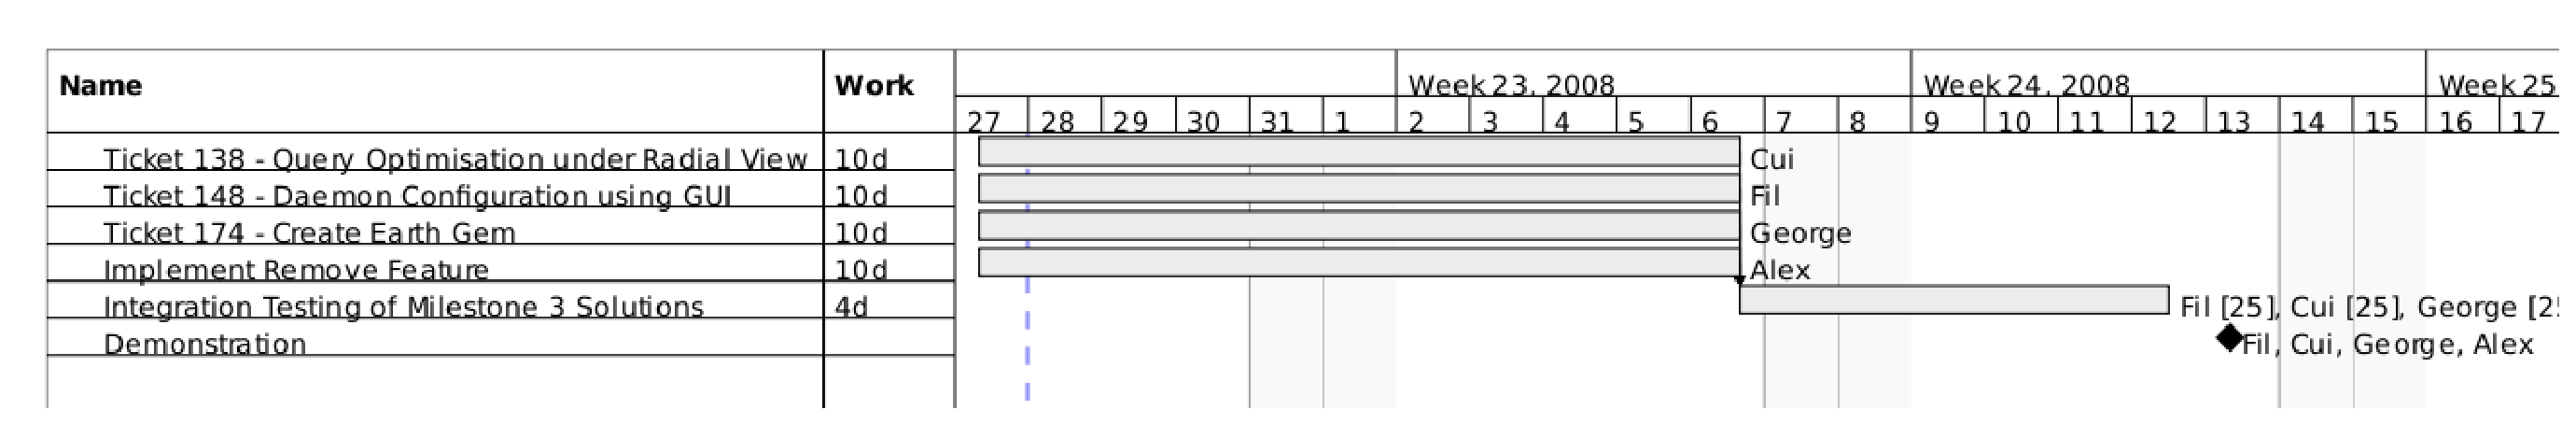
\includegraphics[width=150mm]{figs/m3}
\end{centering}
\caption{Gantt chart of tasks for milestone 3}
\label{fig:m3gannt}
\end{figure}

\newpage

\subsection{Resource Allocation}
 
As described in Section \ref{subsec:purpose-and-scope}, people will be allocated to each task in the following fashion:
 
\begin{itemize}
  
\item \textbf{Ticket 138:} Xiaodong Cui \\
 
\item \textbf{Ticket 148:} Filimoni Lutunaika \\
 
\item \textbf{Ticket 174:} George Sainsbury \\
 
\item \textbf{Earth Remove Feature:} Alex Egan \\
 
\end{itemize}
 
If a task is completed early, or it is noted that less people are required to complete a task on schedule, they will be reallocated to other tasks.\\
 

\subsection{Source Control}

\subsubsection{Task Completion Criteria}

\noindent To ensure the successful integration of each allocation tasks into the group repository, the member responsible will have to make sure that at least one of the other group members can successfully duplicate the end results or outcome of the task.

\paragraph{}
\noindent Upon satisfying the above requirement, the member responsible can then make a pull request to the group's gitHub leader to upload the solution onto the group's git repository for the actual integration testing of the group's collective solutions. 


\subsubsection{Git Repository Process}

\noindent Each group member is expected to follow the git repository procedures outlined in the \emph{Repository Process Document for Earth}.
 

\subsubsection{Testing Process}
\noindent Each group member is expected to follow the testing process procedures outlined in the \emph{Testing Process Document for Earth}.


\subsection{Administration}

In addition to the assigned tasks for this Milestone 1, the roles of Git Leader and Documentation Person will be rotated amongst the Group 1 members at every milestone. This will help to ensure that each member gets a chance to take on extra responsibilities with the view of broadening their individual skills as a software developer.

\subsubsection{Git Leader}

For Milestone 3, Alex will be in charge of managing the repository for Group 1. This includes ensuring that the Milestone 3 solutions undergo integration testing before being commited onto the Group 1 repository.


\subsubsection{Documentation Person}

For Milestone 3, Fil will oversee the documentation requirements for Group 1, which mainly includes setting meeting agendas and organising progress update meetings.

\newpage

\section{References}
 
Sommerville, I. \textit{Software Engineering}, 8th Edition,  Addison-Wesley, 2007\\
\newline
Wikipedia, \textit{Agile software development} Retrieved from \emph{http://en.wikipedia.org/wiki/Agile\_software\_development} on 27/05/2008.\\
\newline
Earth Project, \textit{Ticket 138} Retrieved from \emph{http://open.rsp.com.au/projects/earth/ticket/138} on 27/05/2008.\\
\newline
Earth Project, \textit{Ticket 148} Retrieved from \emph{http://open.rsp.com.au/projects/earth/ticket/148} on 27/05/2008.\\
\newline
Earth Project, \textit{Ticket 174} Retrieved from \emph{http://open.rsp.com.au/projects/earth/ticket/174} on 27/05/2008.\\
\newline
Egan, A and Bamogaddam, M.,\textit{Testing Process Document for Earth} Egan, A and Bamogaddam, M., First Edition, 2008.\\
\newline
Egan, A and Bamogaddam, M.,\textit{Repository Process Document for Earth}  First Edition, 2008.\\

\paragraph{}

\[ END\]
\end{document}
